\documentclass[aspectratio=1610,t]{beamer}

\usepackage[english]{babel}
\usepackage{hyperref}
\usepackage{minted}
\usepackage{alltt}
\usepackage{amsmath}
\usepackage{graphicx}
\usepackage{xcolor}

\usetheme{metropolis}
\usemintedstyle{xcode}
\definecolor{codebg}{RGB}{247, 247, 246}
\setbeamercolor{background canvas}{bg=white}
\hypersetup{colorlinks,linkcolor=,urlcolor=orange}

\title{Lecture 1: Hello, Rust!}
\date{February 1, 2022}
\author{Alexander Stanovoy}
\institute{alex.stanovoy@gmail.com}

\begin{document}

% ----------------------------------------------------------------- %

\begin{frame}
\maketitle
\end{frame}

% ----------------------------------------------------------------- %

\begin{frame}[c]
\frametitle{What is this course about?}
The Rust programming language, its basic and advanced features.
\begin{itemize}
    \item Basics: syntax, collections, traits...
    \item Some nightly features, such as trait specialization.
    \item Parallel and concurrent computing.
    \item Metaprogramming.
    \item Tooling around language.
    \item System safety.
\end{itemize}
\end{frame}

% ----------------------------------------------------------------- %

\begin{frame}[c]
\frametitle{Prerequisites}
\begin{itemize}
    \item Solid knowledge of C++, including C++20 standard.
    \item Understanding of parallel computing and concurrency.
    \item Comprehension of computer architecture and operating systems.
    \item Passion for backend engineering.
\end{itemize}
\end{frame}

% ----------------------------------------------------------------- %

\begin{frame}[c]
\centering\Huge\textbf{Are you ready? :)}
\end{frame}

% ----------------------------------------------------------------- %

\begin{frame}[c]
\centering\Huge\textbf{The creation of Rust: Short history background}
\end{frame}

% ----------------------------------------------------------------- %

\begin{frame}
\frametitle{A brief history of programming languages}
\textbf{Machine codes}

Pros:
\begin{itemize}
    \item Direct execution of code written by engineer.
    \item Don't require any runtime.
\end{itemize}

Cons:
\begin{itemize}
    \item Easy to make a mistake when "typing".
    \item Very hard to read.
    \item Difficult to debug.
    \item Hard to reuse existing code.
    \item Requires a lot of time to write even a simple program.
    \item Code changes from machine to machine.
\end{itemize}
\end{frame}

% ----------------------------------------------------------------- %

\begin{frame}
\frametitle{A brief history of programming languages}
\textbf{Assembly language}

Pros:
\begin{itemize}
    \item Direct execution of the code written by an engineer.
    \item Don't require any runtime.
    \item Not possible to type a nonexistent command or write an incorrect offset.
    \item Mnemonics are easier to read than machine codes.
\end{itemize}

Cons:
\begin{itemize}
    \item Difficult to debug.
    \item Still hard to write complex logic.
    \item Hard to reuse existing code.
    \item Requires a lot of time to write even a simple program.
    \item Usually still requires code changes from machine to machine.
\end{itemize}
\end{frame}

% ----------------------------------------------------------------- %

\begin{frame}
\frametitle{A brief history of programming languages}
\textbf{C language}

Pros:
\begin{itemize}
\item Don't require any runtime.
\item Provides a thin layer of abstraction, allowing to write complex but still readable code: structures, functions, pointers...
\item Abstraction over hardware.
\end{itemize}

Cons:
\begin{itemize}
\item Segfaults, buffer overflows, null pointers, data races, \textbf{undefined behavior}...
\item Not very productive lacks syntax sugar.
\item No unified build system and dependency management.
\end{itemize}
\end{frame}

% ----------------------------------------------------------------- %

\begin{frame}[fragile]
\frametitle{Remember dreadful undefined behaviour?}
\textbf{CVE-2008-0166}

Bug in \texttt{glibc} that resulted in vulnerability in OpenSSL.

\begin{itemize}
    \item \texttt{srandom()} - set seed for non-cryptographic pseudorandom number generator.
    \item If read from \texttt{/dev/random} failed, the following code is executed:
\end{itemize}

\begin{minted}{C}
  struct timeval tv;
  unsigned long junk;
  gettimeofday(&tv, NULL);
  srandom((getpid() << 16) ^ tv.tv_sec ^ tv.tv_usec ^ junk);
\end{minted}

\end{frame}

% ----------------------------------------------------------------- %

\begin{frame}[fragile]
\frametitle{Remember dreadful undefined behaviour?}
\textbf{CVE-2008-0166}

Bug in \texttt{glibc} that resulted in vulnerability in OpenSSL.

\begin{itemize}
    \item \texttt{srandom()} - set seed for non-cryptographic pseudorandom number generator.
    \item If read from \texttt{/dev/random} failed, the following code is executed:
\end{itemize}

\begin{minted}{C}
  struct timeval tv;
  unsigned long junk;
  gettimeofday(&tv, NULL);
  srandom((̶g̶e̶t̶p̶i̶d̶(̶)̶ ̶<̶<̶ ̶1̶6̶)̶ ̶^̶ ̶t̶v̶.̶t̶v̶_̶s̶e̶c̶ ̶^̶ ̶t̶v̶.̶t̶v̶_̶u̶s̶e̶c̶ ^ junk);
\end{minted}

One day, the compiler decided to remove everything except junk :D

\end{frame}

% ----------------------------------------------------------------- %

\begin{frame}[fragile]
\frametitle{Remember dreadful memory unsafety?}
\textbf{Memory unsafety}

\begin{itemize}
    \item Code has full access to memory of the whole process.
    \item Side effects can be unpredictable.
\end{itemize}

\begin{minted}{C}
  char line[1024];
  ssize_t len = getline(&line, sizeof(line), stdin);  
\end{minted}

\end{frame}

% ----------------------------------------------------------------- %

\begin{frame}[fragile]
\frametitle{Remember dreadful memory unsafety?}
\textbf{A story about \texttt{memcpy}}

\begin{minted}{C}
  void *memcpy(void *dest, const void *src, size_t n);
\end{minted}

\end{frame}

% ----------------------------------------------------------------- %

\begin{frame}[fragile]
\frametitle{Remember dreadful memory unsafety?}
\textbf{A story about \texttt{memcpy}}

\begin{minted}{C}
  void *memcpy(void *dest, const void *src, size_t n);
\end{minted}

The \texttt{memcpy()} function copies \texttt{n} bytes from memory area \texttt{src} to memory area \texttt{dest}. The memory areas must not overlap.

\end{frame}

% ----------------------------------------------------------------- %

\begin{frame}[fragile]
\frametitle{Remember dreadful memory unsafety?}
\textbf{A story about \texttt{memcpy}}

\begin{minted}{C}
  void *memcpy(void *dest, const void *src, size_t n);
\end{minted}

The \texttt{memcpy()} function copies \texttt{n} bytes from memory area \texttt{src} to memory area \texttt{dest}. The memory areas must not overlap.

\begin{itemize}
    \item Summer 2010: software developers from Intel added a patch to \texttt{glibc}. Now \texttt{memcpy()} sometimes can copy from right to left.
    \item September 29, 2010: Fedora Linux user found a bug - Flash Player cracks instead of playing sound.
\end{itemize}

\end{frame}

% ----------------------------------------------------------------- %

\begin{frame}[fragile]
\frametitle{Remember dreadful memory unsafety?}
\textbf{A story about \texttt{memcpy}: Who is at fault?}

The only stupidity is crap software violating well known rules that have existed forever.
\begin{flushright}
    \textit{Andreas Schwab, \texttt{glibc} developer}
\end{flushright}

You can call it "crap software" all you like, but the thing is, if \texttt{memcpy} doesn't warn about overlaps, there's no test coverage, and in that case, even well-designed software will have bugs.
\begin{flushright}
    \textit{Linus Torvalds}
\end{flushright}

\end{frame}

% ----------------------------------------------------------------- %

\begin{frame}
\frametitle{A brief history of programming languages}
\textbf{C++ language}

Pros:
\begin{itemize}
    \item Don't require any runtime.
    \item Provides a thick layer of abstraction, allowing to write complex readable code: classes, templates, lambda functions, iterators...
    \item Abstraction over hardware and memory due to OOP.
\end{itemize}

Cons:
\begin{itemize}
    \item Segfaults, buffer overflows, null pointers, data races, \textbf{undefined behaviour}...
    \item Сluttered standard with a lot of gaps due to previous decisions.
    \item No unified build system and dependency management.
\end{itemize}
\end{frame}

% ----------------------------------------------------------------- %

\begin{frame}[fragile]
\frametitle{Remember dreadful undefined behaviour?}
\textbf{An example of regular C++'s UB}

\begin{minted}{cpp}
  std::vector<std::string> createStrings() {
    // Some code
  }

  for (char c : createStrings().at(0)) {
    // undefined behaviour
  }
\end{minted}
\end{frame}

% ----------------------------------------------------------------- %

\begin{frame}[fragile]
\frametitle{I love C++!}
Fun fact: it will not be fixed until C++26 because the proposal in C++23 was rejected.

\begin{center}
    
\includegraphics[width=\textwidth,height=7cm,keepaspectratio]{images/cpp-meme.jpg}
\end{center}
\end{frame}

% ----------------------------------------------------------------- %

\begin{frame}
\frametitle{A brief history of programming languages}
In the meantime: languages such as garbage collection.

\textbf{Java, C\# and similar languages}

Pros:
\begin{itemize}
    \item Require runtime but execution is quite fast due to JIT.
    \item In general, provide thick layer of abstraction.
    \item Run code everywhere where runtime exists.
    \item Safer than C, C++ or similar languages, but implementation-defined and unspecified behavior exist.
\end{itemize}
\end{frame}

% ----------------------------------------------------------------- %

\begin{frame}
\frametitle{A brief history of programming languages}
In the meantime: languages with garbage collection.

\textbf{Java, C\# and similar languages}

Cons:\footnote{\href{https://reberhardt.com/cs110l/spring-2020/slides/lecture-01.pdf}{CS110L Lecture 1 Slides.}}
\begin{itemize}
    \item Expensive: no matter what type of garbage collection is used, there will always be nontrivial memory overhead.
    \item Disruptive: drop what you're doing - it's time for GC!
    \item Non-deterministic: when will the next GC pause be? Who knows! It depends on how much memory is being used.
\end{itemize}
\end{frame}

% ----------------------------------------------------------------- %

\begin{frame}
\frametitle{Garbage Collection cons}
\href{https://discord.com/blog/why-discord-is-switching-from-go-to-rust}{Why Discord is swithing from Go to Rust?}

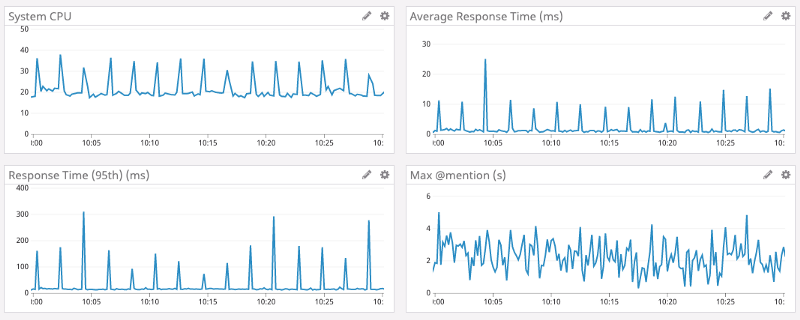
\includegraphics[width=\textwidth,height=\textheight,keepaspectratio]{images/discord-spikes.png}

\end{frame}

% ----------------------------------------------------------------- %

\begin{frame}
\frametitle{Garbage Collection cons}
\href{https://engineering.linkedin.com/blog/2016/02/eliminating-large-jvm-gc-pauses-caused-by-background-io-traffic}{Eliminating Large JVM GC Pauses Caused by Background IO Traffic}

In our production environments, we have seen unexplainable significant STW pauses (> 5 seconds) in our mission-critical Java applications.

\begin{flushright}\textit{LinkedIn Engineering}\end{flushright}

\end{frame}

% ----------------------------------------------------------------- %

\begin{frame}
\frametitle{A brief history of programming languages}
In the meantime: languages with garbage collection.

\textbf{Java, C\# and similar languages}

Cons:
\begin{itemize}
    \item Precludes manual optimization: in some situations, you may want to structure your data in memory in a specific way to achieve high cache performance. GC can't know how you will use memory, so it optimizes for the average use case.
    \item Have poor interoperability.
    \item \textbf{Are not suitable for system programming.}\footnote{Actually suitable, but GC limits use cases.}
\end{itemize}
\end{frame}

% ----------------------------------------------------------------- %

\begin{frame}
\frametitle{A brief history of programming languages}
\textbf{What is system programming?}

System programming - the process of creation of programs that communicate with hardware and other programs, not users.

Examples:
\begin{itemize}
    \item Operating systems, firmware.
    \item Databases: PostgreSQL, MySQL
    \item Virtual machines: JVM, CLR.
    \item Browsers and their engines: Blink, WebKit, Servo.
\end{itemize}
\end{frame}

% ----------------------------------------------------------------- %

\begin{frame}
\frametitle{A brief history of programming languages}
\textbf{What is system programming?}

System programming - the process of creation of programs that communicate with hardware and other programs, not users.

Usual properties:
\begin{itemize}
    \item Fast execution time with stable latency.
    \item High sensitivity to bugs.
    \item High security.
\end{itemize}

At the same time, we try to pursue two goals: performance and safety.
\end{frame}

% ----------------------------------------------------------------- %

\begin{frame}
\frametitle{A brief history of programming languages}
Why is C still used for system programming?

\begin{itemize}
    \item Assembly is "strictly better" than Machine codes.
    \item C is nearly "strictly better" than Assembly.
    \item C++ \textbf{is not} "strictly better" than C.
    \item Languages with runtime \textbf{is not} "strictly better" than C.
\end{itemize}

Will there be a language "strictly better" than C?
\end{frame}

% ----------------------------------------------------------------- %

\begin{frame}
\frametitle{A brief history of programming languages}
\textbf{Rust language}

Pros:
\begin{itemize}
    \item Don't require any runtime.
    \item Provides a thick layer of abstraction, allowing to write complex readable code: structures, generics, traits, closures, iterators...
    \item \textbf{No memory unsafety and undefined behavior.}\footnote{Unless you or your dependencies use \texttt{unsafe} incorrectly.}
    \item Modern standard without any\footnote{There exist not good decisions.} incorrect decisions.
    \item Unified build system and dependency management.
\end{itemize}

According to \href{https://www.zdnet.com/article/microsoft-70-percent-of-all-security-bugs-are-memory-safety-issues/}{Microsoft} and \href{https://www.chromium.org/Home/chromium-security/memory-safety}{Chromium}, ~70\% of bugs involve memory unsafety.
\end{frame}

% ----------------------------------------------------------------- %

\begin{frame}
\frametitle{A brief history of programming languages}
\textbf{Rust language}

Cons:
\begin{itemize}
    \item Difficult to use and especially learn.
    \item Compiled, thus no such simple coding as in, for instance, Python.
    \item If you're using a lot of optimizations or writing software that frequently works with pointers, you'll have to use \textbf{a lot} of \texttt{unsafe}. It may be inconvenient.
\end{itemize}
\end{frame}

% ----------------------------------------------------------------- %

\begin{frame}
\frametitle{What is safety after all?}

Let's take a look at \href{run:code/vector.c}{C code of simple vector} and find some bugs on it to intuitively understand the Rust's features.

\end{frame}

% ----------------------------------------------------------------- %

\begin{frame}[fragile]
\frametitle{What is safety after all?}
\textbf{Dangling pointers}

\begin{minted}{C}
  Vec* vec_new() {
      Vec vec;
      vec.data = NULL;
      vec.length = 0;
      vec.capacity = 0;
      return &vec;
  }
\end{minted}

\end{frame}

% ----------------------------------------------------------------- %

\begin{frame}[fragile]
\frametitle{What is safety after all?}
\textbf{Dangling pointers}

\begin{minted}[escapeinside=||]{C}
  Vec* vec_new() {
      Vec vec;
      vec.data = NULL;
      vec.length = 0;
      vec.capacity = 0;
      |\colorbox{yellow}{return &vec;}|
  }
\end{minted}

Wouldn't it be nice if the compiler realized that \textt{vec} "lives" within those two curly braces, and therefore its address shouldn't be returned from the function?

\end{frame}

% ----------------------------------------------------------------- %

\begin{frame}[fragile]
\frametitle{What is safety after all?}
\textbf{Double frees}

\begin{minted}{C}
  void main() {
      Vec *vec = vec_new();

      /* ... */

      free(vec->data);
      vec_free(vec);
  }
\end{minted}

\end{frame}

% ----------------------------------------------------------------- %

\begin{frame}[fragile]
\frametitle{What is safety after all?}
\textbf{Double frees}

\begin{minted}[escapeinside=||]{C}
  void main() {
      Vec *vec = vec_new();

      /* ... */

      free(vec->data);
      |\colorbox{yellow}{vec\_free(vec);}|
  }
\end{minted}

Wouldn't it be nice if the compiler enforced that free is called on a variable, that variable can no longer be used?

\end{frame}

% ----------------------------------------------------------------- %

\begin{frame}[fragile]
\frametitle{What is safety after all?}
\textbf{Iterator Invalidation}

\begin{minted}{C}
  void main() {
      /* ... */

      int *n = &vec->data[0];
      vec_push(vec, 110);
      printf("%d\n", *n);

      /* ... */
  }
\end{minted}

\end{frame}

% ----------------------------------------------------------------- %

\begin{frame}[fragile]
\frametitle{What is safety after all?}
\textbf{Iterator Invalidation}

\begin{minted}[escapeinside=||]{C}
  void main() {
      /* ... */

      int *n = &vec->data[0];
      vec_push(vec, 110);
      const char* format = "%d\n";
      |\colorbox{yellow}{printf(format, *n);}| // I'm sorry for 'format'

      /* ... */
  }
\end{minted}

Wouldn't it be nice if the compiler stopped us from modifying the data \texttt{n} was pointing to (as it does in \texttt{vec\_push})?

\end{frame}

% ----------------------------------------------------------------- %

\begin{frame}[fragile]
\frametitle{What is safety after all?}
\textbf{Memory leaks}

\begin{minted}{C}
  void vec_push(Vec *vec, int n) {
      if (vec->length == vec->capacity) {
          /* ... */
    
          vec->data = new_data;
          vec->capacity = new_capacity;
      }
    
      /* ... */
  }
\end{minted}

\end{frame}

% ----------------------------------------------------------------- %

\begin{frame}[fragile]
\frametitle{What is safety after all?}
\textbf{Memory leaks}

\begin{minted}[escapeinside=||]{C}
  void vec_push(Vec *vec, int n) {
      if (vec->length == vec->capacity) {
          /* ... */
    
          |\colorbox{yellow}{vec->data = new\_data;}|
          vec->capacity = new_capacity;
      }
    
      /* ... */
  }
\end{minted}

Wouldn't it be nice if the compiler noticed when a piece of heap data no longer had anything pointing to it? (and so then could easily be freed?)

\end{frame}

% ----------------------------------------------------------------- %

\begin{frame}[fragile]
\frametitle{Is Rust safe?}
Rust is theoretically proven to be safe.\\

\begin{tabular}{cl}  
\begin{tabular}{c}

\includegraphics[height=5cm, width=3.5cm]{images/ralf-jung.jpeg}
\end{tabular}
& \begin{tabular}{l}
\parbox{0.5\linewidth}{
    \href{https://www.ralfj.de/research/thesis.html}{Understanding and Evolving the Rust Programming Language, Ralf Jung, August 2020.}

    Awards:
    \begin{itemize}
        \item 2021 Otto Hahn Medal.
        \item Honorable Mention for the 2020 ACM Doctoral Dissertation Award.
        \item 2021 ETAPS Doctoral Dissertation Award.
    \end{itemize}
}
\end{tabular}  \\
\end{tabular}
\end{frame}

% ----------------------------------------------------------------- %

\begin{frame}[fragile]
\frametitle{Is Rust safe?}
RustBelt - formal model of Rust that includes core conceptions of language (borrowing, lifetimes, lifetime inclusion).

\begin{itemize}
    \item Proof of safety of Safe\footnote{There exists Unsafe Rust, but we will return to it later.} Rust.
    \item Definition of sufficiency conditions for every type \texttt{T} to consider it safe abstraction.
    \item Proof of soundness using Coq + Iris: \texttt{Cell}, \texttt{RefCell}, \texttt{thread::spawn}, \texttt{rayon::join}, \texttt{Mutex}, \texttt{RwLock}, \texttt{Arc}.
\end{itemize}
\end{frame}

% ----------------------------------------------------------------- %

\begin{frame}
\frametitle{A brief history of Rust\footnote{\href{https://www.youtube.com/watch?v=79PSagCD_AY}{The History of Rust} talk.}}

\begin{enumerate}
    \item \textbf{(2006-2010)} Started at Mozilla by Graydon Hoare as a personal project.
    \item \textbf{(2010-2012)} Rust is now a Mozilla project.
    \begin{itemize}
        \item The team slowly grows allowing Rust to grow faster.
        \item The aim is to make language that can catch critical mistakes before code even compiles.
    \end{itemize}
    \item \textbf{(2012-2014)} Rust improves type system.
    \begin{itemize}
        \item To make the language safe, the team thought they need a garbage collector, but they figured out they don't need it: everything can be done in the level of type system!
        \item Birth of Cargo - the Rust package manager. Influenced by \texttt{ruby} and \texttt{npm}.
    \end{itemize}
    \item \textbf{(2014-present)} Rust grows!
\end{enumerate}
\end{frame}

% ----------------------------------------------------------------- %

\begin{frame}
\frametitle{Is it popular of just a niche language?}
\textbf{Google}

\begin{itemize}
    \item \href{https://security.googleblog.com/2021/04/rust-in-linux-kernel.html}{Pushing Rust to Linux Kernel.}
    \item \href{https://fuchsia.dev/fuchsia-src/development/languages/rust}{Developing new OS Fuchsia in Rust.}\footnote{\href{https://imgur.com/gknVmYk}{Count of lines of code in different languages.}}
    \item \href{https://security.googleblog.com/2021/04/rust-in-android-platform.html}{Enabled support of Rust in Android.}
\end{itemize}

\textbf{Meta} \footnote{\href{https://engineering.fb.com/2021/04/29/developer-tools/rust/}{A brief history of Rust at Facebook}}

\begin{itemize}
    \item Mononoke - version control system.
    \item Diem - blockchain.
    \item Metaverse - virtual reality.
\end{itemize}
\end{frame}

% ----------------------------------------------------------------- %

\begin{frame}
\frametitle{Is it popular of just a niche language?}
\textbf{Amazon}\footnote{\href{https://aws.amazon.com/blogs/opensource/how-our-aws-rust-team-will-contribute-to-rusts-future-successes/}{How our AWS Rust team will contribute to Rust’s future successes.}}

\begin{itemize}
    \item Hired core developers of Tokio (the most popular framework for async).
    \item \href{https://github.com/firecracker-microvm/firecracker}{Firecracker} - open source virtualization technology.
    \item \href{https://github.com/bottlerocket-os/bottlerocket}{Bottlerocket OS} - open-source Linux-based operating system meant for hosting containers.
    \item \href{https://aws.amazon.com/ec2/nitro/}{Nitro} - compute environments; underlying platform for Amazon EC2.
\end{itemize}

\textbf{Microsoft}

\begin{itemize}
    \item \href{https://msrc-blog.microsoft.com/2019/11/07/using-rust-in-windows/}{Rewrited Windows component in Rust}.
    \item \href{https://github.com/microsoft/windows-rs}{Official Rust WinAPI wrapper.}
\end{itemize}
\end{frame}

% ----------------------------------------------------------------- %

\begin{frame}
\frametitle{Why companies sometimes do \textbf{not} use Rust?}

\begin{itemize}
    \item Already wrote a lot of code in another language.
    \item Company's internal tools do not support Rust, and maintenance could be costly.
    \item In a big company, you should have your committee to help support language in the company. 
    \item Hard to find developers in such a difficult and fresh language.
    \item Rust developers are usually talented people with high salary expectations.
\end{itemize}
\end{frame}

% ----------------------------------------------------------------- %

\begin{frame}
\frametitle{Why companies sometimes do \textbf{not} use Rust?}

\begin{itemize}
    \item Already wrote a lot of code in another language.
    \item Company's internal tools do not support Rust, and maintenance could be costly.
    \item In a big company, you should have your committee to help support language in the company. 
    \item Hard to find developers in such a difficult and fresh language.
    \item Rust developers are usually talented people with high salary expectations.
\end{itemize}

At the same time, startups and small companies do not hesitate to use the language.

\textit{*Silly blockchain joke*}.
\end{frame}

% ----------------------------------------------------------------- %

\begin{frame}[c]
\centering\Huge\textbf{Finally some Rust}
\end{frame}

% ----------------------------------------------------------------- %

\begin{frame}[fragile]
\frametitle{First of all: Hello, World!}

How to write Hello World in Rust?

\begin{minted}{rust}
    fn main() {
        println!("Hello, World!");
    }
\end{minted}
\end{frame}

% ----------------------------------------------------------------- %

\begin{frame}[fragile]
\frametitle{First of all: Hello, World!}

How to write Hello World in Rust?

\begin{minted}{rust}
    fn main() {
        println!("Hello, World!");
    }
\end{minted}

\begin{minted}{bash}
    $ rustc main.rs  # no optimizations
    $ ./main
    Hello, World!
\end{minted}
\end{frame}

% ----------------------------------------------------------------- %

\begin{frame}[fragile]
\frametitle{First of all: Hello, World!}

How to write Hello World in Rust: assembly edition.

\begin{minted}[fontsize=\small]{rust}
    #![no_main]

    #[link_section=".text"]
    #[no_mangle]
    pub static main: [u32; 9] = [
        3237986353,
        3355442993,
        120950088,
        822083584,
        252621522,
        1699267333,
        745499756,
        1919899424,
        169960556,
    ];
\end{minted}
\end{frame}

% ----------------------------------------------------------------- %

\begin{frame}[fragile]
\frametitle{First of all: defining variables}
\textbf{Integer variable types:}

\begin{table}[]
\begin{tabular}{|l|l|l|l|l|l|l|}
\hline
Bits count & 8  & 16  & 32  & 64  & 128  & 32/64 \\ \hline
Signed     & \texttt{i8} & \texttt{i16} & \texttt{i32} & \texttt{i64} & \texttt{i128} & \texttt{isize} \\ \hline
Unsigned   & \texttt{u8} & \texttt{u16} & \texttt{u32} & \texttt{u64} & \texttt{u128} & \texttt{usize} \\ \hline
\end{tabular}
\end{table}

\texttt{usize} - size of the pointer.
\end{frame}

% ----------------------------------------------------------------- %

\begin{frame}[fragile]
\frametitle{First of all: defining variables}
To define a variable, use \texttt{let} keyword:

\begin{minted}{rust}
    let idx: usize = 92;
\end{minted}

Literals:

\begin{minted}{rust}
    let y = 92_000_000i64;
    let hex_octal_bin = 0xffff_ffff + 0o777 + 0b1;
\end{minted}

In Rust there's \textbf{type inference}. For integer type, the default type is \texttt{i32}.

Variables are \textbf{immutable} by default. To make a variable mutable, use \texttt{mut} keyword:

\begin{minted}{rust}
    let mut idx: usize = 0x1022022;
\end{minted}
\end{frame}

% ----------------------------------------------------------------- %

\begin{frame}[fragile]
\frametitle{First of all: defining variables}
Floats and bools: \texttt{f32}, \texttt{f64} and \texttt{bool}.

In Rust, \texttt{bool} can have only two values: \texttt{true} and \texttt{false}:

\begin{minted}{rust}
    let mut x = true;
    x = false;
    // error: expected `bool`, found integer!
    // x = 1;
\end{minted}

At the same time, it's 1 byte in memory (will be important later).


\end{frame}

% ----------------------------------------------------------------- %

\begin{frame}[fragile]
\frametitle{Arithmetic}
\begin{itemize}
    \item Basic arithmetic: \texttt{+}, \texttt{-}, \texttt{*}, \texttt{/}, \texttt{\%}
    \item \texttt{/}, \texttt{\%} round to 0.
\begin{minted}{rust}
    let (x, y) = (15, -15);
    let (a1, b1) = (x / -4, x % -4);
    let (a2, b2) = (y /  4, y %  4);
    // outputs "-3 3 and -3 -3"
    println!("{a1} {b1} and {a2} {b2}");
\end{minted}
    \item Bitwise and logical operations \texttt{!}, \texttt{<<}, \texttt{>>}, \texttt{|}, \texttt{\&}
    \item No \texttt{++}
    \item Functions \texttt{(-92i32).abs()}, \texttt{0b001100u8.count\_ones()}, \texttt{2i32.pow(10)} ans so on.
    \item \href{https://doc.rust-lang.org/book/appendix-02-operators.html}{Full list of operators here.}
\end{itemize}
\end{frame}

% ----------------------------------------------------------------- %

\begin{frame}[fragile]
\frametitle{Type casting}
In Rust, there's no type implicit casting:

\begin{minted}[fontsize=\small]{rust}
    let x: u16 = 1;

    // error: mismatched types
    // let y: u32 = x;

    // Just filling leading bits with zeros
    let z: u16 = y as u16;
    let y: u32 = x.into();

    // Cutting leading zeros
    let to_usize = 92u64 as usize;
    let from_usize = 92usize as u64;
\end{minted}

\texttt{as} - explicit casting operator.
\end{frame}

% ----------------------------------------------------------------- %

\begin{frame}[fragile]
\frametitle{Type casting}
\textbf{Note}: Casting is not transitive, that is, even if:

\begin{minted}{rust}
    e as U1 as U2
\end{minted}

Is a valid expression, the expression:

\begin{minted}{rust}
    e as U2
\end{minted}

It is not necessarily so.
\end{frame}

% ----------------------------------------------------------------- %

\begin{frame}[fragile]
\frametitle{Overflow}
Overflow is a programmer's mistake. In debug build vs in release build:

\begin{minted}[fontsize=\small]{rust}
    fn main() {
        let x = i32::max_value();
        let y = x + 1;
        println!("{}", y);
    }
\end{minted}

\begin{minted}[fontsize=\small]{bash}
    $ cargo run
    thread 'main' panicked at 'attempt to add with overflow',
    main.rs:3:13

    $ cargo run --release
    -2147483648
\end{minted}
\end{frame}

% ----------------------------------------------------------------- %

\begin{frame}[fragile]
\frametitle{Explicit arithmetic}
\begin{minted}[fontsize=\small]{rust}
    let x = i32::MAX;

    let y = x.wrapping_add(1);
    assert_eq!(y, i32::MIN);

    let y = x.saturating_add(1);
    assert_eq!(y, i32::MAX);

    let (y, overflowed) = x.overflowing_add(1);
    assert!(overflowed);
    assert_eq!(y, i32::MAX)

    match x.checked_add(1) {
        Some(y) => unreachable!(),
        None => println!("overflowed"),
    }
\end{minted}
\end{frame}

% ----------------------------------------------------------------- %

\begin{frame}[fragile]
\frametitle{Floating point}
\begin{minted}{rust}
    let y = 0.0f32; // Litaral f32
    let x = 0.0;    // Default value

    // Point is necessary
    // error: expected f32, found integer variable
    // let z: f32 = 0;
    let z = 0.0f32;

    let not_a_number = std::f32::NAN;
    let inf = std::f32::INFINITY;

    // Wow, so many functions!
    8.5f32.ceil().sin().round().sqrt()
\end{minted}
\end{frame}

% ----------------------------------------------------------------- %

\begin{frame}[fragile]
\frametitle{Boolean}
\begin{minted}{rust}
    let to_be = true;
    let not_to_be = !to_be;
    let the_question = to_be || not_to_be;
\end{minted}

\texttt{\&\&} and \texttt{||} are lazy.
\end{frame}

% ----------------------------------------------------------------- %

\begin{frame}[fragile]
\frametitle{Tuple}
\begin{minted}[fontsize=\small]{rust}
    let pair: (f32, i32) = (0.0, 92);
    let (x, y) = pair;
    // The same as this
    // Note the shadowing!
    let x = pair.0;
    let y = pair.1;

    let void_result = println!("hello");
    assert_eq!(void_result, ());

    let trailing_comma = (
        "Archibald",
        "Buttle",
    );
\end{minted}
\end{frame}

% ----------------------------------------------------------------- %

\begin{frame}[fragile]
\frametitle{More on shadowing}
What is the output of this code?

\begin{minted}{rust}
    let x = 10;
    for i in 0..5 {
        if x == 10 {
            println!("{i}");
            let x = 12;
        }
    }
\end{minted}
\end{frame}

% ----------------------------------------------------------------- %

\begin{frame}[fragile]
\frametitle{More on shadowing}
What is the output of this code?

\begin{minted}{rust}
    let x = 10;
    for i in 0..5 {
        if x == 10 {
            let x = 12;
            println!("{i} {x}");
        }
    }
    // This code outputs 0 10\n1 10\n2 10\n3 10\n4 10\n
\end{minted}
\end{frame}

% ----------------------------------------------------------------- %

\begin{frame}[fragile]
\frametitle{More on shadowing}
Drop is compiler optimization. \href{https://rust.godbolt.org/z/3b5hfr7db}{Godbolt}.

\begin{minted}{rust}
    pub fn shadowing(num: i32) -> i32 {
        let vec = vec![0, 1, 2, 3];
        let vec = vec![4, 5, 6, 7];
        vec[0]
    }
\end{minted}
\end{frame}

% ----------------------------------------------------------------- %

\begin{frame}[fragile]
\frametitle{Tuple}
\begin{minted}{rust}
    // Zero element tuple, or Unit
    let x = ();
    let y = {};
    assert!(x == y); // OK

    // One element tuple
    let x = (42,);
\end{minted}
\end{frame}

% ----------------------------------------------------------------- %

\begin{frame}[fragile]
\frametitle{Tuple}
In memory, tuple is stored continuously.

\begin{table}[]
\begin{tabular}{|l|l|}
\hline
\texttt{7}        & \texttt{07 00 00 00}             \\ \hline
\texttt{(7, 263)} & \texttt{07 00 00 00 07 01 00 00} \\ \hline
\end{tabular}
\end{table}
\end{frame}

% ----------------------------------------------------------------- %

\begin{frame}[fragile]
\frametitle{Tuple}
Tuple is a zero-cost abstraction!

\begin{minted}{rust}
    let t = (92,);
    // 0x7ffc6b2f6aa4
    println!("{:?}", &t as *const (i32,));
    // 0x7ffc6b2f6aa4
    println!("{:?}", &t.0 as *const i32);
\end{minted}

Meanwhile in Python:

\begin{minted}{py}
    t = (92,)
    print(id(t))     # 139736506707248
    print(id(t[0]))  # 139736504680928
\end{minted}
\end{frame}

% ----------------------------------------------------------------- %

\begin{frame}[fragile]
\frametitle{Tuple}
Tuple is a zero-cost abstraction!

\begin{minted}{rust}
    let t = (92,);
    // 0x7ffc6b2f6aa4
    println!("{:?}", &t as *const (i32,));
    // 0x7ffc6b2f6aa4
    println!("{:?}", &t.0 as *const i32);
\end{minted}

Meanwhile in Python:

\begin{minted}{py}
    t = (92,)
    print(id(t))     # 139736506707248
    print(id(t[0]))  # 139736504680928
\end{minted}
\end{frame}

% ----------------------------------------------------------------- %

\begin{frame}[fragile]
\frametitle{Array}
\begin{minted}{rust}
    let xs: [u8; 3] = [1, 2, 3];
    assert_eq!(xs[0], 1);    // index -- usize
    assert_eq!(xs.len(), 3); // len() -- usize

    let mut buf = [0u8; 1024];
\end{minted}

The size of an array is a constant known at compile-time and the part of the type.
\end{frame}

% ----------------------------------------------------------------- %

\begin{frame}[fragile]
\frametitle{References}
\begin{itemize}
    \item Is really a pointer in compiled program.
    \item Cannot be \texttt{NULL}.
    \item Guaranties that the object is alive.
    \item There are \textt{\&} and \textt{\&mut} references.
\end{itemize}

\begin{minted}{rust}
    let mut x: i32 = 92;
    let r: &mut i32 = &mut 92; // Reference created explicitly
    *r += 1;                   // Explicit dereference
\end{minted}
\end{frame}

% ----------------------------------------------------------------- %

\begin{frame}[fragile]
\frametitle{References}
In C++ we have to use \texttt{std::reference\_wrapper} to store a reference in a vector:

\begin{minted}{cpp}
    int x = 10;
    std::vector<std::reference_wrapper<int>> v;
    v.push_back(x);
\end{minted}

In Rust, references are a first class objects so we can push them to vector directly:

\begin{minted}{rust}
    let x = 10;
    let mut v = Vec::new();
    v.push(&x);
\end{minted}
\end{frame}

% ----------------------------------------------------------------- %

\begin{frame}[fragile]
\frametitle{Pointers}
\begin{itemize}
    \item Useless without \textt{unsafe}, because you cannot dereference it.
    \item Can be NULL.
    \item Does not guarrantee that the object is alive.
    \item \textbf{Very rarely needed}. Examples: FFI, some data structures, optimizations...
\end{itemize}

\begin{minted}{rust}
    let x: *const i32 = std::ptr::null();
    let mut y: *const i32 = std::ptr::null();
    let z: *mut i32 = std::ptr::null_mut();
    let mut t: *mut i32 = std::ptr::null_mut();
\end{minted}

In Rust, we read type names from left to right, not from right to left like in C++:

\begin{minted}{cpp}
    uint32_t const * const x = nullptr;
    uint32_t const * y = nullptr;
    uint32_t* const z = nullptr;
    uint32_t* t = nullptr;
\end{minted}
\end{frame}

% ----------------------------------------------------------------- %

\begin{frame}[fragile]
\frametitle{Box}
\begin{itemize}
    \item Pointer to some data on the heap.
    \item Pretty like C++'s \texttt{std::unique\_ptr}, but without \texttt{NULL}
\end{itemize}

\begin{minted}{rust}
    let x: Box<i32> = Box::new(92);
\end{minted}
\end{frame}

% ----------------------------------------------------------------- %

\begin{frame}[fragile]
\frametitle{Functions}
Functions are defined via \texttt{fn} keyword. Note the expressions and statements!

\begin{minted}[fontsize=\small]{rust}
    fn func1() {}
    fn func2() -> () {}
    fn func3() -> i32 {
        0
    }
    fn func4(x: u32) -> u32 {
        return x;
    }
    fn func5(x: u32, mut y: u64) -> u64 {
        y = x as u64 + 10;
        return y
    }
    fn func6(x: u32, mut y: u64) -> u32 {
        x + 10
    }
\end{minted}
\end{frame}

% ----------------------------------------------------------------- %

\begin{frame}[fragile]
\frametitle{More on expressions and statements}
This works in any other scope, for instance in \texttt{if}'s:

\begin{minted}{rust}
    let y = 42;
    let x = if y < 42 {
        345
    } else {
        y + 534
    }
\end{minted}
\end{frame}

% ----------------------------------------------------------------- %

\begin{frame}[fragile]
\frametitle{Structures}
Structures are defined via \texttt{struct} keyword:

\begin{minted}[fontsize=\small]{rust}
    struct Example {
        oper_count: usize,
        data: Vec<i32>, // Note the trailing comma
    }
\end{minted}

Rust \textbf{do not} give any guarantees about memory representation by default. Even these structures can be different in memory!

\begin{minted}[fontsize=\small]{rust}
    struct A {
        x: Example,
    }

    struct B {
        y: Example,
    }
\end{minted}
\end{frame}

% ----------------------------------------------------------------- %

\begin{frame}[fragile]
\frametitle{Structures}
Let's add new methods to \texttt{Example}:

\begin{minted}[fontsize=\small]{rust}
    impl Example {
        // Associated
        pub fn new() -> Self {
            Self {
                oper_count: 0,
                data: Vec::new(),
            }
        }
    
        pub fn push(&mut self, x: i32) {
            self.oper_count += 1;
            self.data.push(x)
        }

        /* Next slide */
    }    
\end{minted}
\end{frame}

% ----------------------------------------------------------------- %

\begin{frame}[fragile]
\frametitle{Structures}
Let's add new methods to \texttt{Example}:

\begin{minted}[fontsize=\small]{rust}
    impl Example {
        /* Previous slide */

        pub fn oper_count(&self) -> usize {
            self.oper_count
        }
    
        pub fn eat_self(self) {
            println!("later on lecture :)")
        }
    }
\end{minted}

Note: you can have multiple \texttt{impl} blocks.
\end{frame}

% ----------------------------------------------------------------- %

\begin{frame}[fragile]
\frametitle{Structures}
Initialize a structure and use it:

\begin{minted}{rust}
    let mut x = Example {
        oper_count: 0,
        data: Vec::new(),
    };
    let y = Example::new();
    x.push(10);
    assert_eq!(x.oper_count(), 1);
\end{minted}
\end{frame}

% ----------------------------------------------------------------- %

\begin{frame}[fragile]
\frametitle{Simple example of generics}
What about being \textit{generic} over arguments?

\begin{minted}{rust}
    struct Example<T> {
        oper_count: usize,
        data: Vec<T>,
    }
\end{minted}
\end{frame}

% ----------------------------------------------------------------- %

\begin{frame}[fragile]
\frametitle{Simple example of generics}
What about being \textit{generic} over arguments?

\begin{minted}[fontsize=\small]{rust}
    impl<T> Example<T> {
        pub fn new() -> Self {
            Self {
                oper_count: 0,
                data: Vec::new(),
            }
        }

        pub fn push(&mut self, x: T) {
            self.oper_count += 1;
            self.data.push(x)
        }

        /* The rest is the same */
    } 
\end{minted}
\end{frame}

% ----------------------------------------------------------------- %

\begin{frame}[fragile]
\frametitle{Simple example of generics}
Initialize a structure and use it:

\begin{minted}[fontsize=\small]{rust}
    let mut x = Example<i32> {
        oper_count: 0,
        data: Vec::new(),
    };
    let y = Example::<i32>::new(); // ::<> called 'turbofish'
    let z: Example<i32> = Example {
        oper_count: 0,
        data: Vec::new(),
    };
    let z: Example::<i32> = Example { // Wow, this works too?!
        oper_count: 0,
        data: Vec::new(),
    };
    x.push(10);
    assert_eq!(x.oper_count(), 1);
\end{minted}
\end{frame}

% ----------------------------------------------------------------- %

\begin{frame}[fragile]
\frametitle{Conditions and loops: \texttt{if}, \texttt{while}, \texttt{for}, \texttt{loop}}
\begin{minted}{rust}
    let mut x = 2;
    if x == 2 { // No braces in Rust
        x += 2;
    }
    while x > 0 { // No braces too
        x -= 1;
        println!("{x}");
    }
\end{minted}
\end{frame}

% ----------------------------------------------------------------- %

\begin{frame}[fragile]
\frametitle{Conditions and loops: \texttt{if}, \texttt{while}, \texttt{for}, \texttt{loop}}
\begin{minted}{rust}
    loop { // Just loop until 'return', 'break' or never return.
        println!("I'm infinite!");
        x += 1;
        if x == 10 {
            println!("I lied...");
            // Note no ;
            break
            // But this will go too
            // break;
        }
    }
\end{minted}
\end{frame}

% ----------------------------------------------------------------- %

\begin{frame}[fragile]
\frametitle{Conditions and loops: \texttt{if}, \texttt{while}, \texttt{for}, \texttt{loop}}
In Rust, we can break with a value from \texttt{while} and \texttt{loop}!

\begin{minted}{rust}
    let mut counter = 0;
    let result = loop {
        counter += 1;
        if counter == 10 {
            break counter * 2;
        }
    };
    assert_eq!(result, 20);
\end{minted}

Default \texttt{break} is just \texttt{break ()}.
\end{frame}

% ----------------------------------------------------------------- %

\begin{frame}[fragile]
\frametitle{Conditions and loops: \texttt{if}, \texttt{while}, \texttt{for}, \texttt{loop}}
Or break on outer \texttt{while}, \texttt{for} or \texttt{loop}:

\begin{minted}[fontsize=\small]{rust}
    'outer: loop {
        println!("Entered the outer loop");
        'inner: for _ in 0..10 {
            println!("Entered the inner loop");

            // This would break only the inner loop
            // break;

            // This breaks the outer loop
            break 'outer;
        }
        println!("This point will never be reached");
    }
    println!("Exited the outer loop");
\end{minted}
\end{frame}

% ----------------------------------------------------------------- %

\begin{frame}[fragile]
\frametitle{Conditions and loops: \texttt{if}, \texttt{while}, \texttt{for}, \texttt{loop}}
Time for \texttt{for} loops!

\begin{minted}{rust}
    for i in 0..10 {
        println!("{i}");
    }
    for i in 0..=10 {
        println!("{i}");
    }
    for i in [1, 2, 3, 4] {
        println!("{i}");
    }
\end{minted}
\end{frame}

% ----------------------------------------------------------------- %

\begin{frame}[fragile]
\frametitle{Conditions and loops: \texttt{if}, \texttt{while}, \texttt{for}, \texttt{loop}}
Time for \texttt{for} loops!

\begin{minted}{rust}
    let vec = vec![1, 2, 3, 4];
    for i in &vec { // By reference
        println!("{i}");
    }
    for i in vec { // Consumes vec; will be discussed later
        println!("{i}");
    }
\end{minted}
\end{frame}

% ----------------------------------------------------------------- %

\begin{frame}[fragile]
\frametitle{Enumerations}
Enumerations are one of the best features in Rust :)

\begin{minted}{rust}
    enum MyEnum {
        First,
        Second,
        Third, // Once again: trailing comma
    }
    enum OneMoreEnum<T> {
        Ein(i32),
        Zwei(u64, Example<T>),
    }

    let x = MyEnum::First;
    let y: MyEnum = MyEnum::First;
    let z = OneMoreEnum::Zwei(42, Example::<usize>::new());
\end{minted}
\end{frame}

% ----------------------------------------------------------------- %

\begin{frame}[fragile]
\frametitle{Enumerations: Option and Result}
In Rust, there's two important enums in \texttt{std}, used for error handling:

\begin{minted}{rust}
    enum Option<T> { // 'Maybe' from functional languages
        Some(T),
        None,
    }

    enum Result<T, E> {
        Ok(T),
        Err(E),
    }
\end{minted}

We will discuss them a bit later in the course.
\end{frame}

% ----------------------------------------------------------------- %

\begin{frame}[fragile]
\frametitle{Match}
\texttt{match} is one of things that will help you to work with \texttt{enum}.

\begin{minted}{rust}
    let x = MyEnum::First;
    match x {
        MyEnum::First => println!("First"),
        MyEnum::Second => {
            for i in 0..5 { println!("{i}"); }
            println!("Second");
        },
        _ => println!("Matched something!"),
    }
\end{minted}
\end{frame}

% ----------------------------------------------------------------- %

\begin{frame}[fragile]
\frametitle{The \texttt{\_} symbol}
\begin{itemize}
    \item \texttt{\_} matches everything in \texttt{match} (called wildcard).
    \item Used for inference sometimes:
    \begin{minted}{rust}
    // Rust does not know here to what type
    // you want to collect
    let mut vec: Vec<_> = (0..10).collect();
    vec.push(42u64);
    \end{minted}
    \item And to make a variable unused:
    \begin{minted}{rust}
    let _x = 10;
    // No usage of _x, no warnings!
    \end{minted}
\end{itemize}
\end{frame}

% ----------------------------------------------------------------- %

\begin{frame}[fragile]
\frametitle{Match}
\texttt{match} can match multiple objects at a time:

\begin{minted}{rust}
    let x = OneMoreEnum::<i32>::Ein(2);
    let y = MyEnum::First;
    match (x, y) {
        (OneMoreEnum::Ein(x), MyEnum::First) => {
            println!("Hello!");
        },
        // Destructuring
        (OneMoreEnum::Zwei(a, _), _) => println!("{a}"),
        _ => println!("oooof!"),
    }
\end{minted}
\end{frame}

% ----------------------------------------------------------------- %

\begin{frame}[fragile]
\frametitle{Match}
There's feature to match different values with same code:

\begin{minted}{rust}
    let number = 13;
    match number {
        1 => println!("One!"),
        2 | 3 | 5 | 7 | 11 => println!("This is a prime"),
        13..=19 => println!("A teen"),
        _ => println!("Ain't special"),
    }
\end{minted}
\end{frame}

% ----------------------------------------------------------------- %

\begin{frame}[fragile]
\frametitle{Match}
And we can apply some additional conditions called guards:

\begin{minted}{rust}
    let pair = (2, -2);
    println!("Tell me about {:?}", pair);
    match pair {
        (x, y) if x == y => println!("These are twins"),
        // The ^ `if condition` part is a guard
        (x, y) if x + y == 0 => println!("Antimatter, kaboom!"),
        (x, _) if x % 2 == 1 => println!("The first one is odd"),
        _ => println!("No correlation..."),
    }
\end{minted}
\end{frame}

% ----------------------------------------------------------------- %

\begin{frame}[fragile]
\frametitle{Match}
Match is an expression too:

\begin{minted}{rust}
    let boolean = 13;
    let x = match boolean {
        13 if foo() => 0,
        // You have to cover all of the possible cases
        13 => 1,
        _ => 2,
    };
\end{minted}
\end{frame}

% ----------------------------------------------------------------- %

\begin{frame}[fragile]
\frametitle{Match}
Ignoring the rest of the tuple:

\begin{minted}[fontsize=\small]{rust}
    let triple = (0, -2, 3);
    println!("Tell me about {:?}", triple);
    match triple {
        (0, y, z) => {
            println!("First is `0`, `y` is {y}, and `z` is {z}")
        },
        // `..` can be used to ignore the rest of the tuple
        (1, ..) => {
            println!("First is `1` and the rest doesn't matter"),
        },
        _ => {
            println!("It doesn't matter what they are"),
        },
    }
\end{minted}
\end{frame}

% ----------------------------------------------------------------- %

\begin{frame}[fragile]
\frametitle{Match}
Let's define a struct:

\begin{minted}[fontsize=\small]{rust}
    struct Foo {
        x: (u32, u32),
        y: u32,
    }

    let foo = Foo { x: (1, 2), y: 3 };
\end{minted}
\end{frame}

% ----------------------------------------------------------------- %

\begin{frame}[fragile]
\frametitle{Match}
Destructuring the struct:

\begin{minted}{rust}
    match foo {
        Foo { x: (1, b), y } => {
            println!("First of x is 1, b = {},  y = {} ", b, y);
        },
        Foo { y: 2, x: i } => {
            println!("y is 2, i = {:?}", i);
        },
        Foo { y, .. } => { // ignoring some variables:
            println!("y = {}, we don't care about x", y)
        },
        // error: pattern does not mention field `x`
        // Foo { y } => println!("y = {}", y),
    }
\end{minted}
\end{frame}

% ----------------------------------------------------------------- %

\begin{frame}[fragile]
\frametitle{Match}
Binding values to names:

\begin{minted}{rust}
    match age() {
        0 => println!("I haven't celebrated my birthday yet"),
        n @ 1..=12 => println!("I'm a child of age {n}"),
        n @ 13..=19 => println!("I'm a teen of age {n}"),
        n => println!("I'm an old person of age {n}"),
    }
\end{minted}
\end{frame}

% ----------------------------------------------------------------- %

\begin{frame}[fragile]
\frametitle{Match}
Binding values to names + arrays:

\begin{minted}{rust}
    let s = [1, 2, 3, 4];
    let mut t = &s[..]; // or s.as_slice()
    loop {
        match t {
            [head, tail @ ..] => {
                println!("{head}");
                t = &tail;
            }
            _ => break,
        }  
    } // outputs 1\n2\n\3\n4\n
\end{minted}
\end{frame}

% ----------------------------------------------------------------- %

\begin{frame}[fragile]
\frametitle{Enumerations}
You can create custom functions for \texttt{enum}:

\begin{minted}{rust}
    enum Test {
        A(i32),
        B,
    }

    impl Test {
        pub fn unwrap(self) -> i32 {
            match self {
                Self::A(x) => x,
                Self::B => panic!("error!"),
            }
        }
    }
\end{minted}
\end{frame}

% ----------------------------------------------------------------- %

\begin{frame}[fragile]
\frametitle{\texttt{if let}}
Sometimes we need only one enumeration variant to do something. Can we write it in a better way?

\begin{minted}{rust}
    let optional = Some(7);
    match optional {
        Some(i) => {
            println!("It's Some({i})");
        },
        _ => {},
        // ^ Required because `match` is exhaustive
    };
\end{minted}
\end{frame}

% ----------------------------------------------------------------- %

\begin{frame}[fragile]
\frametitle{\texttt{if let}}
Sometimes we need only one enumeration variant to do something. Can we write it in a better way?

\begin{minted}{rust}
    let optional = Some(7);
    if let Some(i) = optional {
        println!("It's Some({i})");
    }
\end{minted}
\end{frame}

% ----------------------------------------------------------------- %

\begin{frame}[fragile]
\frametitle{\texttt{while let}}
Same with \texttt{while}:

\begin{minted}{rust}
    let mut optional = Some(0);
    while let Some(i) = optional {
        if i > 9 {
            println!("Greater than 9, quit!");
            optional = None;
        } else {
            println!("`i` is `{i}`. Try again.");
            optional = Some(i + 1);
        }
    }
\end{minted}
\end{frame}

% ----------------------------------------------------------------- %

\begin{frame}[fragile]
\frametitle{Enumerations}
Let's dive into details and compare enumerations with C++ \texttt{enum} and \texttt{union}.

\begin{itemize}
    \item To identify the variant, we store some \textit{bits} in fields of enum. These bits are called \textit{discriminant}.
    \item The count of bits is exactly as many as needed to keep the number of variants.
    \item These bits are stored in unused bits of enumeration in another field. (compiler optimizations!)
    \item That means we have something like \texttt{union} and \texttt{enum} in C++ at the same time! (Note: in Rust there's \texttt{union}, we'll dive into it later)
\end{itemize}
\end{frame}

% ----------------------------------------------------------------- %

\begin{frame}[fragile]
\frametitle{Enumerations}

\begin{minted}{rust}
    enum Test {
        First(bool),
        Second,
        Third,
        Fourth,
    }
    assert_eq!(
        std::mem::size_of::<Test>(), 1
    );
    assert_eq!(
        std::mem::size_of::<Option<Box<i32>>>(), 8
    );
\end{minted}
\end{frame}

% ----------------------------------------------------------------- %

\begin{frame}[fragile]
\frametitle{Enumerations}
\begin{minted}{rust}
    enum Test1 {
        First(bool, bool),
        Field0,
        // More fields...
        Field253,
    }
    enum Test2 {
        First(bool, bool),
        Field0,
        // More fields...
        Field254,
    }
    assert_eq!(std::mem::size_of::<Test1>(), 2);
    assert_eq!(std::mem::size_of::<Test2>(), 3);
\end{minted}
\end{frame}

% ----------------------------------------------------------------- %

\begin{frame}[fragile]
\frametitle{Vector}
Dynamic array, just like in C++.

\begin{minted}{rust}
    pub struct Vec<T> {
        ptr: *const T,
        length: usize,
        capacity: usize,
        // PhantomData<T>?
    }
\end{minted}
\end{frame}

% ----------------------------------------------------------------- %

\begin{frame}[fragile]
\frametitle{Vector}
\begin{minted}{rust}
    use std::mem::size_of;
    assert_eq!(
        size_of::<Vec<i32>>(),
        size_of::<usize>() * 3,
    );

    let mut xs = vec![1, 2, 3];
    // To declare vector with same element and
    // specific count of elements, write
    // vec![42; 113];
    xs.push(4);
    assert_eq!(xs.len(), 4);
    assert_eq!(xs[2], 3);
\end{minted}
\end{frame}

% ----------------------------------------------------------------- %

\begin{frame}[fragile]
\frametitle{Slices}
We can create a slice to a vector or array. A slice is a contiguous sequence of elements in a collection.

\begin{minted}{rust}
    let a = [1, 2, 3, 4, 5];
    let slice1 = &a[1..4];
    let slice2 = &slice1[..2];
    assert_eq!(slice1, &[2, 3, 4]);
    assert_eq!(slice2, &[2]);
\end{minted}
\end{frame}

% ----------------------------------------------------------------- %

\begin{frame}[fragile]
\frametitle{Panic!}
In Rust, when we encounter an unrecoverable error, we \texttt{panic!}

\begin{minted}{rust}
    let x = 42;
    if x == 42 {
        panic!("The answer!")
    }
\end{minted}

There are some useful macros that \texttt{panic!}

\begin{itemize}
    \item \texttt{unimplemented!}
    \item \texttt{unreachable!}
    \item \texttt{todo!}
    \item \texttt{assert!}
    \item \texttt{assert\_eq!}
\end{itemize}
\end{frame}

% ----------------------------------------------------------------- %

\begin{frame}[fragile]
\frametitle{\texttt{println!}}
The best tool for debugging, we all know. 

\begin{minted}[fontsize=\small]{rust}
    let x = 42;
    println!("{x}");
    println!("The value of x is {}, and it's cool!", x);
    println!("{:04}", x); // 0042
    println!("{value}", value=x); // 42
    let vec = vec![1, 2, 3];
    println!("{vec:?}"); // [1, 2, 3]
    println!("{:?}", vec);
    let y = (100, 200);
    println!("{:#?}", (100, 200));
    // (
    //     100,
    //     200,
    // )
\end{minted}
\end{frame}

% ----------------------------------------------------------------- %

\begin{frame}[fragile]
\frametitle{\texttt{Inhabited type \texttt{!}}}
Rust always requires to return something correct.

\begin{minted}{rust}
    // error: mismatched types
    // expected `i32`, found `()`
    fn func() -> i32 {}
\end{minted}

How does this code work?

\begin{minted}{rust}
    fn func() -> i32 {
        unimplemented!("not ready yet")
    }
\end{minted}
\end{frame}

% ----------------------------------------------------------------- %

\begin{frame}[fragile]
\frametitle{\texttt{Inhabited type \texttt{!}}}
Rust always requires to return something correct.

\begin{minted}{rust}
    // error: mismatched types
    // expected `i32`, found `()`
    fn func() -> i32 {}
\end{minted}

How does this code work?

\begin{minted}{rust}
    fn func() -> i32 {
        unimplemented!("not ready yet")
    }
\end{minted}

\textbf{Return type that is never constructed}: \texttt{!}.
\end{frame}

% ----------------------------------------------------------------- %

\begin{frame}[fragile]
\frametitle{\texttt{Inhabited type \texttt{!}}}
\textbf{Return type that is never constructed}: \texttt{!}

Same as:

\begin{minted}{rust}
    enum Test {} // empty, could not be constructed
\end{minted}

\texttt{loop} without any \texttt{break} returns \texttt{!}
\end{frame}

% ----------------------------------------------------------------- %

\begin{frame}
\center\Huge\textbf{Borrow Checker}


\includegraphics[height=6cm,keepaspectratio]{images/check-failed.jpeg}
\end{frame}

% ----------------------------------------------------------------- %

\begin{frame}[fragile]
\frametitle{What's the problem, Rust?}
\begin{minted}{rust}
    let mut v = vec![1, 2, 3];
    let x = &v[0];
    v.push(4);
    println!("{}", x);
\end{minted}
\end{frame}

% ----------------------------------------------------------------- %

\begin{frame}[fragile]
\frametitle{What's the problem, Rust?}
\begin{minted}{rust}
    let mut v = vec![1, 2, 3];
    let x = &v[0];
    v.push(4);
    println!("{}", x);
\end{minted}

\begin{minted}{bash}
error[E0502]: cannot borrow `v` as mutable because it is also
borrowed as immutable
 --> src/main.rs:8:5
  |
7 |     let x = &v[0];
  |              - immutable borrow occurs here
8 |     v.push(4);
  |     ^^^^^^^^^ mutable borrow occurs here
9 |     println!("{}", x);
  |                    - immutable borrow later used here
\end{minted}
\end{frame}

% ----------------------------------------------------------------- %

\begin{frame}[fragile]
\frametitle{What's the problem, Rust?}
\begin{minted}{rust}
    fn sum(v: Vec<i32>) -> i32 {
        let mut result = 0;
        for i in v {
            result += i;
        }
        result
    }

    fn main() {
        let mut v = vec![1, 2, 3];
        println!("first sum: {}", sum(v));
        v.push(4);
        println!("second sum: {}", sum(v))
    }
\end{minted}
\end{frame}

% ----------------------------------------------------------------- %

\begin{frame}[fragile]
\frametitle{What's the problem, Rust?}
\begin{minted}{rust}
error[E0382]: borrow of moved value: `v`
  --> src/main.rs:12:5
   |
10 |     let mut v = vec![1, 2, 3];
   |         ----- move occurs because `v` has type `Vec<i32>`,
   |  which does not implement the `Copy` trait
11 |     println!("first sum: {}", sum(v));
   |                                   - value moved here
12 |     v.push(4);
   |     ^^^^^^^^^ value borrowed here after move
\end{minted}
\end{frame}

% ----------------------------------------------------------------- %

\begin{frame}[fragile]
\frametitle{Ownership rules}
\begin{itemize}
    \item Each value in Rust has a variable that's called it's \textit{owner}.
    \item There can be only one owner at a time.
    \item When the owner goes out of scope, the value will be dropped.
\end{itemize}
\end{frame}

% ----------------------------------------------------------------- %

\begin{frame}[fragile]
\frametitle{Ownership rules}
\begin{minted}{rust}
    fn main() {
        let s = vec![1, 4, 8, 8];
        let u = s;
        println!(“{:?}”, u);
        // This won't compile!
        // println!("{:?}", s);
    }
\end{minted}
\end{frame}

% ----------------------------------------------------------------- %

\begin{frame}[fragile]
\frametitle{Ownership rules}
\begin{minted}[fontsize=\small]{rust}
    fn om_nom_nom(s: Vec<i32>) {
        println!("I have consumed {s:?}");
    }

    fn main() {
        let s = vec![1, 4, 8, 8];
        om_nom_nom(s);
        println!("{s:?}");
    }
\end{minted}

\begin{itemize}
    \item Each "owner" has the responsibility to clean up after itself.
    \item When you move \texttt{s} into \texttt{om\_nom\_nom}, it becomes the owner of \texttt{s}, and it will free \texttt{s} when it’s no longer needed in that scope. \textit{Technically the \texttt{s} parameter in \texttt{om\_nom\_nom} become the owner}.
    \item That means you can no longer use it in \texttt{main}!
    \item In C++, we will create a copy!
\end{itemize}
\end{frame}

% ----------------------------------------------------------------- %

\begin{frame}[fragile]
\frametitle{Ownership rules}
Given what we just saw, how can the following be the valid syntax?

\begin{minted}{rust}
    fn om_nom_nom(n: u32) {
        println!("{} is a very nice number", n);
    }

    fn main() {
        let n: u32 = 110;
        let m = n;
        om_nom_nom(n);
        om_nom_nom(m);
        println!("{}", m + n);
    }
\end{minted}
\end{frame}

% ----------------------------------------------------------------- %

\begin{frame}[fragile]
\frametitle{Ownership rules}
\begin{itemize}
    \item Say you have a group of lawyers that are reviewing and signing a contract over Google Docs (just pretend it's true :) )
    \item What are some ground rules we'd need to set to avoid chaos?
    \item If someone modifies the contract before everyone else reviews/signs it, that's fine.
    \item But if someone modifies the contract while others are reviewing it, people might miss changes and think they're signing a contract that says something else.
    \item We should allow a single person to modify, or everyone to read, but not both.
\end{itemize}
\end{frame}

% ----------------------------------------------------------------- %

\begin{frame}[fragile]
\frametitle{Ownership rules}
\begin{itemize}
    \item Say you have a group of lawyers that are reviewing and signing a contract over Google Docs (just pretend it's true :) )
    \item What are some ground rules we'd need to set to avoid chaos?
    \item If someone modifies the contract before everyone else reviews/signs it, that's fine.
    \item But if someone modifies the contract while others are reviewing it, people might miss changes and think they're signing a contract that says something else.
    \item We should allow a single person to modify, or everyone to read, but not both.
\end{itemize}
\end{frame}

% ----------------------------------------------------------------- %

\begin{frame}[fragile]
\frametitle{Borrowing intuition}
\begin{itemize}
    \item I should be able to have as many "const" pointers to a piece of data that I like.
    \item However, if I have a "non-const" pointer to a piece of data at the same time, this could invalidate what the other const pointers are viewing. (e.g., they can become dangling pointers...)
    \item If I have at most one "non-const" pointer at any given time, this should be OK.
\end{itemize}
\end{frame}

% ----------------------------------------------------------------- %

\begin{frame}[fragile]
\frametitle{Borrowing}
\begin{itemize}
    \item We can have multiple shared (immutable) references at once (with no mutable references) to a value.
    \item We can have only one mutable reference at once. (no shared references to it)
    \item This paradigm pops up a lot in systems programming, especially when you have "readers" and "writers". In fact, you've already studied it in the course of Theory and Practice of Concurrency.
\end{itemize}
\end{frame}

% ----------------------------------------------------------------- %

\begin{frame}[fragile]
\frametitle{Borrowing}
\begin{itemize}
    \item The lifetime of a value starts when it's created and ends the \textit{last time it's used}.
    \item Rust doesn't let you have a reference to a value that lasts longer than the value's lifetime.
    \item Rust computes lifetimes at compile time using static analysis. (this is often an over-approximation!)
    \item Rust calls the special "drop" function on a value once its lifetime ends. (this is essentially a destructor)
\end{itemize}
\end{frame}

% ----------------------------------------------------------------- %

\begin{frame}[fragile]
\frametitle{Drop implementation?}
\begin{minted}{rust}
    let vec = vec![];
    drop(vec);
\end{minted}
\end{frame}

% ----------------------------------------------------------------- %

\begin{frame}[fragile]
\frametitle{Drop implementation?}
\begin{minted}{rust}
    let vec = vec![];
    drop(vec);
\end{minted}

\begin{minted}{rust}
    fn drop(self) {}
\end{minted}
\end{frame}

% ----------------------------------------------------------------- %

\begin{frame}[fragile]
\frametitle{Drop flags}
\begin{minted}{rust}
    let x = Box::new(92);
    let y;
    let z;
    if condition {
        y = x;
    } else {
        z = x;
    }
    // Who cleans the memory?
\end{minted}
\end{frame}

% ----------------------------------------------------------------- %

\begin{frame}[fragile]
\frametitle{Drop flags}
\begin{minted}{rust}
    let x = Box::new(92);
    let y;
    let z;
    if condition {
        y = x;
    } else {
        z = x;
    }
    // Who cleans the memory?
\end{minted}

Invisible flag on the stack: is the variable initialized?
\end{frame}

% ----------------------------------------------------------------- %

\begin{frame}[fragile]
\frametitle{Borrowing}
\begin{minted}{rust}
    let mut x;
    // this access would be illegal, nowhere to
    // draw the flow from:
    // assert_eq!(x, 42);
    x = 42;
    // this is okay, can draw a flow from the
    // value assigned above:
    let y = &x;
    // this establishes a second, mutable flow from x:
    x = 43;
    // this continues the flow from y, which in turn
    // draws from x:
    assert_eq!(*y, 42);
\end{minted}
\end{frame}

% ----------------------------------------------------------------- %

\begin{frame}[fragile]
\frametitle{Borrowing}
\begin{minted}{rust}
    let x1 = 42;
    let y1 = Box::new(84);
    { // starts a new scope
        let z = (x1, y1);
        // z goes out of scope, and is dropped;
        // it in turn drops the values from x1 and y1
    }
    // x1's value is Copy, so it was not moved into z
    let x2 = x1;
    // y1's value is not Copy, so it was moved into z
    // let y2 = y1;
\end{minted}
\end{frame}

% ----------------------------------------------------------------- %

\begin{frame}[fragile]
\frametitle{Conclusion}
\begin{itemize}
    \item We studied why we need Rust and where it's used.
    \item Learned the basics of language syntax.
    \item And passed the borrow check :)
\end{itemize}
\end{frame}

% ----------------------------------------------------------------- %

\end{document}
